\section{Introduction}

Provenance tracking aims to answer questions like ``where did these data come from'', ``why are these data in the output'' and ``how were these data computed''. Program slicing is a collection of techniques for provenance tracking that attempts to take a run of a program and and areas of interest in the output and turn them into the subset of the input and the program that were responsible for generating those specific outputs.

Provenance tracking is important because in order to audit any computational process, we need robust and well-founded notions of provenance to track how data are used, how data are computed, and what data influenced a particular outcome. Existing approaches are often tied to particular programming languages or implementations. In this paper we develop a general categorical approach.

\note{We will use biproducts, and use some results from \cite{karvonen2020}.}

\subsection{Galois Program Slicing}

Perera and collaborators introduced the idea of {\em Galois Program Slicing} as a particular conception of
program slicing for provenance, described in several publications~\cite{perera12a,perera16d,ricciotti17}.
Galois program slicing forms the basis of Perera's data visualisation tool \href{https://f.luid.org/}{Fluid}
that allows interactive exploration of programmatically generated visualisations.

At a high level, Galois Program Slicing assumes that, for each possible value that may be input or output by a program, there exists a lattice of {\em approximations} of that value. For a particular run of a program that takes input $x$ and produces output $y$, we also get a Galois connection between the lattice of approximations of $x$ and the lattice of approximations of $y$. The right half of the Galois connection is the ``forward direction'' taking approximations of the input to approximations of the output; the left half of the Galois connection is the ``backward direction'' that takes approximations of the output to the least (i.e., most approximate) approximation of the input that gives rise to this output approximation.

\begin{example}
  The following program is written in Haskell \cite{haskell} syntax, using a list comprehension to filter a list of pairs of labels and numbers to those numbers with a given label, and then to compute the sum of the numbers:
  \begin{displaymath}
    \begin{array}{l}
      \mathrm{query} :: \mathrm{Label} \to [(\mathrm{Label}, \mathrm{Int})] \to \mathrm{Int} \\
      \mathrm{query}\,l\,\mathit{db} = \mathrm{sum}\,[ n \mid (l',n) \leftarrow \mathit{db}, l \equiv l' ]
    \end{array}
  \end{displaymath}
  With $\mathit{db} = [(\mathsf{a}, 0), (\mathsf{b}, 1), (\mathsf{a}, 1)]$, we will have $\mathit{query}\,\mathsf{a}\,\mathit{db}$ and $\mathit{query}\,\mathsf{b}\,\mathit{db}$ both evaluating to $1$.

  Now suppose that for a given run of the program, we are interested in which of the numerical parts of the input are used to compute the output for the query parameters $l = \mathsf{a}$ and $l = \mathsf{b}$. We can use Galois Program Slicing to do this. We arrange for the approximations of the input to form the following lattice, where the actual piece of data is at the top and information lost by approximation is represented by $\bot$s:
  \begin{center}
    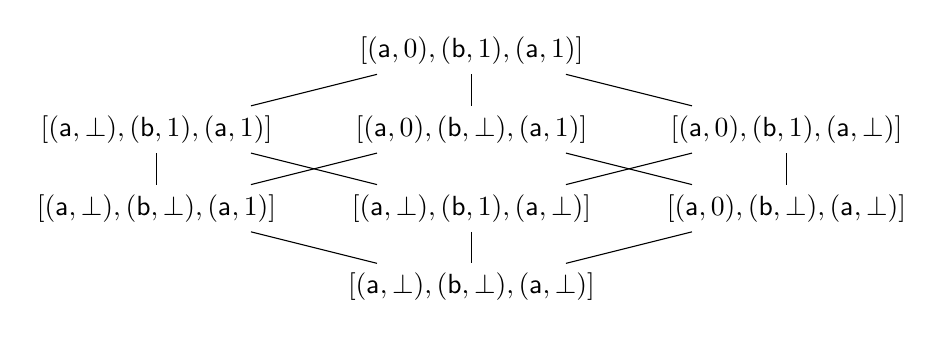
\begin{tikzpicture}
      \node (top) at (0,0) {$[(\mathsf{a}, 0), (\mathsf{b}, 1), (\mathsf{a}, 1)]$};
      % row 2
      \node [below of=top] (ioi) {$[(\mathsf{a}, 0), (\mathsf{b}, \bot), (\mathsf{a}, 1)]$};
      \node [left of=ioi,xshift=-3cm] (oii) {$[(\mathsf{a}, \bot), (\mathsf{b}, 1), (\mathsf{a}, 1)]$};
      \node [right of=ioi,xshift=3cm] (iio) {$[(\mathsf{a}, 0), (\mathsf{b}, 1), (\mathsf{a}, \bot)]$};
      % row 3
      \node [below of=ioi] (oio) {$[(\mathsf{a}, \bot), (\mathsf{b}, 1), (\mathsf{a}, \bot)]$};
      \node [left of=oio,xshift=-3cm] (ooi) {$[(\mathsf{a}, \bot), (\mathsf{b}, \bot), (\mathsf{a}, 1)]$};
      \node [right of=oio,xshift=3cm] (ioo) {$[(\mathsf{a}, 0), (\mathsf{b}, \bot), (\mathsf{a}, \bot)]$};
      % row 4
      \node [below of=oio] (bot) {$[(\mathsf{a}, \bot), (\mathsf{b}, \bot), (\mathsf{a}, \bot)]$};

      % links
      \draw (top) -- (ioi);
      \draw (top) -- (oii);
      \draw (top) -- (iio);
      \draw (ioi) -- (ooi);
      \draw (ioi) -- (ioo);
      \draw (oii) -- (ooi);
      \draw (oii) -- (oio);
      \draw (iio) -- (ioo);
      \draw (iio) -- (oio);
      \draw (ooi) -- (bot);
      \draw (oio) -- (bot);
      \draw (ioo) -- (bot);
    \end{tikzpicture}
  \end{center}
  The output approximation lattice looks like this, where $1$ is the actual data point that was returned in both runs of the program, and $\bot$ indicates that we are approximating this piece of data away:
  \begin{center}
    \begin{tikzpicture}
      \node (top) at (0,0) {$1$};
      \node [below of=top] (bot) {$\bot$};
      \draw (top) -- (bot);
    \end{tikzpicture}
  \end{center}
  These are not the only choices of approximation lattices that we could have taken. For the input, we have chosen a lattice that allows us to ``forget'' (approximate away) numbers in the input, but not any of the other data or the overall structure. However, other choices are also useful. Indeed, one of the aims of this work is to clarify how to choose approximation structure approriate for different tasks by use of type information. We elaborate on this further in Section \todo{XYZ}.

  Galois program slicing associates with each run of the program a Galois connection telling us how the inputs and outputs are related in that run. The backwards portion $\partial (\mathit{query}\,l)_r$ tells us, given an approximation of the output what the least approximation of the input is needed to generate that output. In the case of the two runs considered in this example, if we say we are not interested in the output by feeding in the least approximation $\bot$, then we find that we only need the least approximation of the input:
  \begin{displaymath}
    \partial (\mathit{query}\,l)_r(\bot) = [(\mathsf{a},\bot), (\mathsf{b}, \bot), (\mathsf{a}, \bot)]
  \end{displaymath}
  for both $l = \mathsf{a}$ and $l = \mathsf{b}$. If instead we take the greatest approximation of the output (i.e., the output ``$1$'' itself), then the two query runs' backwards approximations return different results:
  \begin{displaymath}
    \begin{array}{l}
      \partial (\mathit{query}\,\mathsf{a})_r(1) = [(\mathsf{a},0), (\mathsf{b},\bot), (\mathsf{a},1)] \\
      \partial (\mathit{query}\,\mathsf{b})_r(1) = [(\mathsf{a},\bot), (\mathsf{b},1), (\mathsf{a},\bot)]
    \end{array}
  \end{displaymath}
  Pieces of the input that were {\em not} used are replaced by $\bot$. As we expect, the run of the query with label $\mathsf{a}$ depends on the entries in the database labelled with $\mathsf{a}$, and likewise for the run with label $\mathsf{b}$.

  In this case, the forwards portion of the Galois connection tells us for each approximation of the input whether or not it is sufficient to compute the output. In this example, if we provide insufficient data to compute the output, then we will get an underapproximated output. For example, $\partial (\mathit{query}\, \mathsf{a})_f([(\mathsf{a},0),(\mathsf{b},\bot),(\mathsf{a},\bot)]) = \bot$ because we need all the values associated with the label $\mathsf{a}$ to compute their sum.

  In a simple query like this, it is easy to work out the dependency relationship between the input and output. However, the benefit of Galois Program Slicing is that it is {\em automatic} for all programs, no matter how complex the relationship between input and output is. Moreover, by changing what we mean by ``approximation'' we can compute a range of different information about a program.
\end{example}

Previous work on Galois program slicing uses an operational semantics of programs that generates a trace of each execution which can be interpreted after the fact to compute the Galois connection described above. This becomes {\em program slicing} by including the source code of the program as part of the input, so that, in the backward direction, the least approximation of the input required for an output approximation includes the least part of the program required.

\todo{Explain what the plan for the paper is}

\todo{Perhaps more elaboration on the applications of program slicing}

\subsection{Galois Program Slicing and Automatic Differentiation}

\todo{explain why we want a more abstract view on galois program slicing}
There is a close analogy between Galois Program Slicing and Automatic Differentiation for differentiable programs. We have already hinted at this in the description above, but let us now make it explicit.

\begin{itemize}
\item For Galois Program Slicing, we assume that every value has an associated lattice of {\em approximations}. For differentiable programs, every point has an associated vector space of {\em tangents}.
\item For Galois Program Slicing, every program has an associated forward approximation map that takes approximations forward from the input to the output. This map {\em preserves meets}. For differentiable programs, every program has a forward derivative that takes tangents of the input to tangents of the output. The forward derivative map is {\em linear}, so it preserves addition of tangents and the zero tangent.
\item For Galois Program Slicing, every program has an associated backward approximation map that takes approximations of the output back to least approximations of the input. This map {\em preserves joins}. For differentiable programs, every program has a reverse derivative that takes tangents of the output to tangents of the input. This map is again {\em linear}.
\item For Galois Program Slicing, the forward and backward approximation maps are related by being a Galois connection. For differentiable programming, the forward and reverse derivatives are related by being each others' transpose.
\end{itemize}

Given this close connection between Galois program slicing and differentiable programming, we can take structures intended for modelling automatic differentiation and use them to model Galois program slicing. This will enable us to generalise and expand the scope of Galois program slicing to act as a foundation for data provenance in a wide range of computational settings.

\subsection{Outline and Contributions}

Our primary contribution in this article is to elucidate Galois Program Slicing by relating it to differentiable programming and automatic differentiation. In doing so, we aim to expand the applicability of program slicing, and to potentially transfer efficient automatic differentiation implementation techniques from automatic differentiation to program slicing and provenance tracking.

\begin{enumerate}
\item We explain how the CHAD framework of Vákár et al. can be adapted to give a general categorical framework for Galois Program Slicing,
\item Using our adapted CHAD framework, we can explain how type structure can be used to control the approximation lattices associated with data points, something that was ``hard coded'' in previous presentations of Galois Program Slicing.
\item With the benefit of our abstract setting, we can relate Galois Program Slicing to other parts of denotational semantics. In particular, we show that there is a close connection with Stable Domain Theory, a proposed solution to capturing sequentiality by recording more intensional information about programs' sensitivity to approximations.
\item We also relate Galois Program Slicing to categorical treatments of differentiability via Tangent Categories \note{Bob: not sure about this.}
\end{enumerate}
